\chapter{Proposed Methodology}
\label{chap3}

In the previous chapter, we have discussed the theories that support this
research related to the speech processing using MATLAB . In this chapter we will proposed our methodology for this project.\\\\
Basically we are following the given below question step by step.
In this Matlab problem you will see the effects of Decimation \& Interpolation on an
audio signal.\\
Record your speech of about 5 seconds at sampling frequency of 32 kHz.
You can use either �wavrecord()� MATLAB function or windows sound recorder for
this purpose.\\
If you use Sound Recorder, then u need to first set its properties for recording sound
at 32 kHz and single channel.\\
\begin{enumerate}
\item Plot the time and frequency domain magnitude spectrums of this speech signal.
(Use �wavread()� to read the speech signal. Use �freqz()� to plot the frequency
spectrum). What is highest frequency of this signal? Play this signal using
�wavplay()�.
%
\item Decimate the signal by a factor of 2. Again plot the time and frequency domain
spectrum of the signal. Play the sound. What do you observe?
%
\item Again decimate the signal by a factor of 2. Plot the time and frequency domain
spectrum of the signal. Play the sound. What do you observe?
%
\item Now interpolate the signal by a factor of 2. Plot the time and frequency domain
spectrum of the signal. Play the sound. What do you observe?
%
\item Again interpolate the signal by a factor of 2. Plot the time and frequency domain
spectrum of the signal. Play the sound. What do you observe?
%
\end{enumerate}

\section{Block Diagram}
Let us look at the simplified block diagram in Figure \ref{blockDiagram}, which illustrates the main components involved
in recording an audio signal with MATLAB. A microphone converts acoustic sound waves (which are
essentially variations in air pressure over time) into continuous electronic signals (voltages). These
voltages are then filtered using a so-called low-pass filter with cut-off frequency fs/2.\\\\\\
 In non-technical terms, frequencies in the analog voltage signal higher than fs/2 will be removed completely�frequencies
below fs/2 are left untouched. The filtered signal is then sampled at a sampling rate of fs
in a so-called analog-to-digital converter (ADC, for short). Since frequencies higher than fs/2 cannot be represented
when sampling a continuous signals, the low-pass filter is essential in the sampling process. (Maybe you
recall the activity above where you sampled your voice at fs = 32000 Hz; high frequencies were completely
filtered out!) The digitized samples are then transmitted to MATLAB and stored in a vector.
\begin{figure}[H]  %h=positioning
\begin{center}
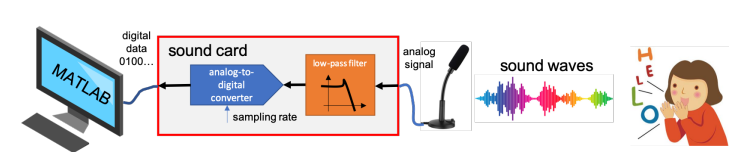
\includegraphics[scale=0.70]{Chapter3/blockDiagram}
\caption{Simplified block diagram of a microphone, sound-card, and computer. The microphone converts
air pressure into voltages, which are filtered and sampled. The samples are then transferred to MATLAB.}
\label{blockDiagram}
\end{center}
\end{figure}

\section{Flow Diagram}
Figure \ref{flowDiagram} shows the flow of the decimate function. In this project decimate function is the main function which we are using to process our signal with different factors.Decimation reduces the original sampling rate for a sequence to a lower rate, the opposite of interpolation. The decimation process filters the input data with a low pass filter and then resamples the resulting smoothed signal at a lower rate.\\\\
y = decimate(x,r) reduces the sample rate of x, the input signal, by a factor of r. The decimated vector, y, is shortened by a factor of r so that \\
\begin{center}
$length(y) = ceil(length\frac{x}{r})$
\end{center}
By default, decimate uses a low pass Chebyshev Type I infinite impulse response (IIR) filter of order 8.
\begin{figure}[H]  %h=positioning
\begin{center}
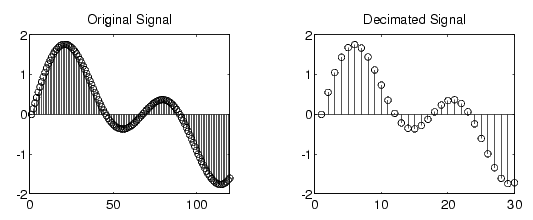
\includegraphics[scale=0.95]{Chapter3/DecimateASignalExample2}
\caption{Example of Decimating A Signal }
\label{DecimateASignalExample}
\end{center}
\end{figure}

\begin{figure}[H]  %h=positioning
\begin{center}
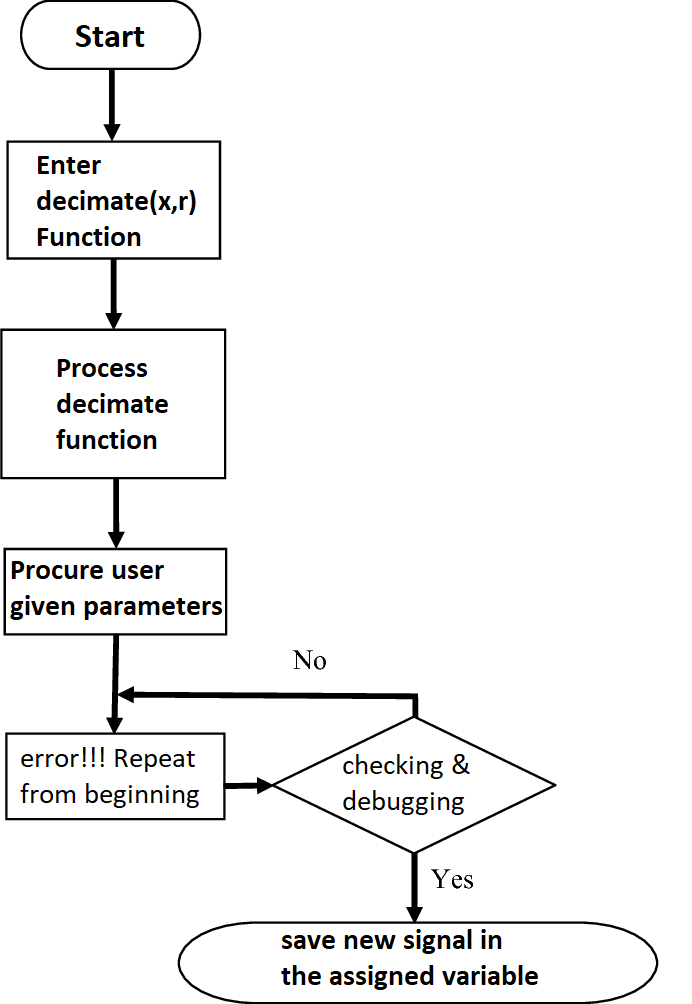
\includegraphics[scale=0.60]{Chapter3/flowDiagram}
\caption{Flow Diagram of the Project}
\label{flowDiagram}
\end{center}
\end{figure}

\section{System Model}
DSP System Toolbox provides algorithms and tools for the design and simulation of signal processing systems. These capabilities are provided as MATLAB functions, MATLAB System objects, and Simulink blocks. The system toolbox includes design methods for specialized FIR and IIR filters, FFTs, multirate processing, and DSP techniques for processing streaming data and creating real-time prototypes.\\\\
You can design adaptive and multirate filters, implement filters using computationally efficient architectures, and simulate floating-point digital filters. Tools for signal I/O from files and devices, signal generation, spectral analysis, and interactive visualization enable you to analyze system behavior and performance. For rapid prototyping and embedded system design, the system toolbox supports fixed-point arithmetic and C or HDL code generation.

\begin{figure}[H]  %h=positioning
\begin{center}
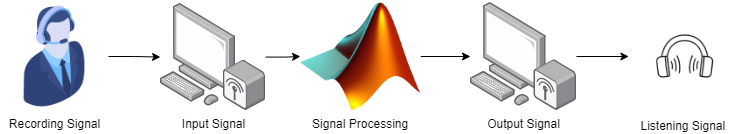
\includegraphics[scale=0.60]{Chapter3/systemModel}
\caption{System Model of the Project}
\label{systemModel}
\end{center}
\end{figure}


\section{Component Selection}
Signal processing engineers use MATLAB and Simulink at all stages of development�from analyzing signals and exploring algorithms to evaluating design implementation tradeoffs for building real-time signal processing systems. MATLAB and Simulink offer:
\begin{enumerate}
\item Built-in functions and apps for analysis and preprocessing of time-series data, spectral and time-frequency analysis, and signal measurements
%
\item Apps and algorithms to design, analyze, and implement digital filters (FIR and IIR) from basic FIR and IIR filters to adaptive, multirate, and multistage designs
%
\item An environment to model and simulate signal processing systems with a combination of programs and block diagrams
%
\item Capabilities to model fixed-point behavior and automatically generate C/C++ or HDL code for deploying on embedded processors, FPGAs, and ASICs
%
\item Tools for developing predictive models on signals and sensor data using machine learning and deep learning workflows
%
\end{enumerate}

{ \small \bfseries Note: Make sure you are using MATLAB 2013 or any less Version because wavrecord, wavplay are being replaced with audiorecorder/getaudiodata.}
\begin{figure}[H]  %h=positioning
\begin{center}
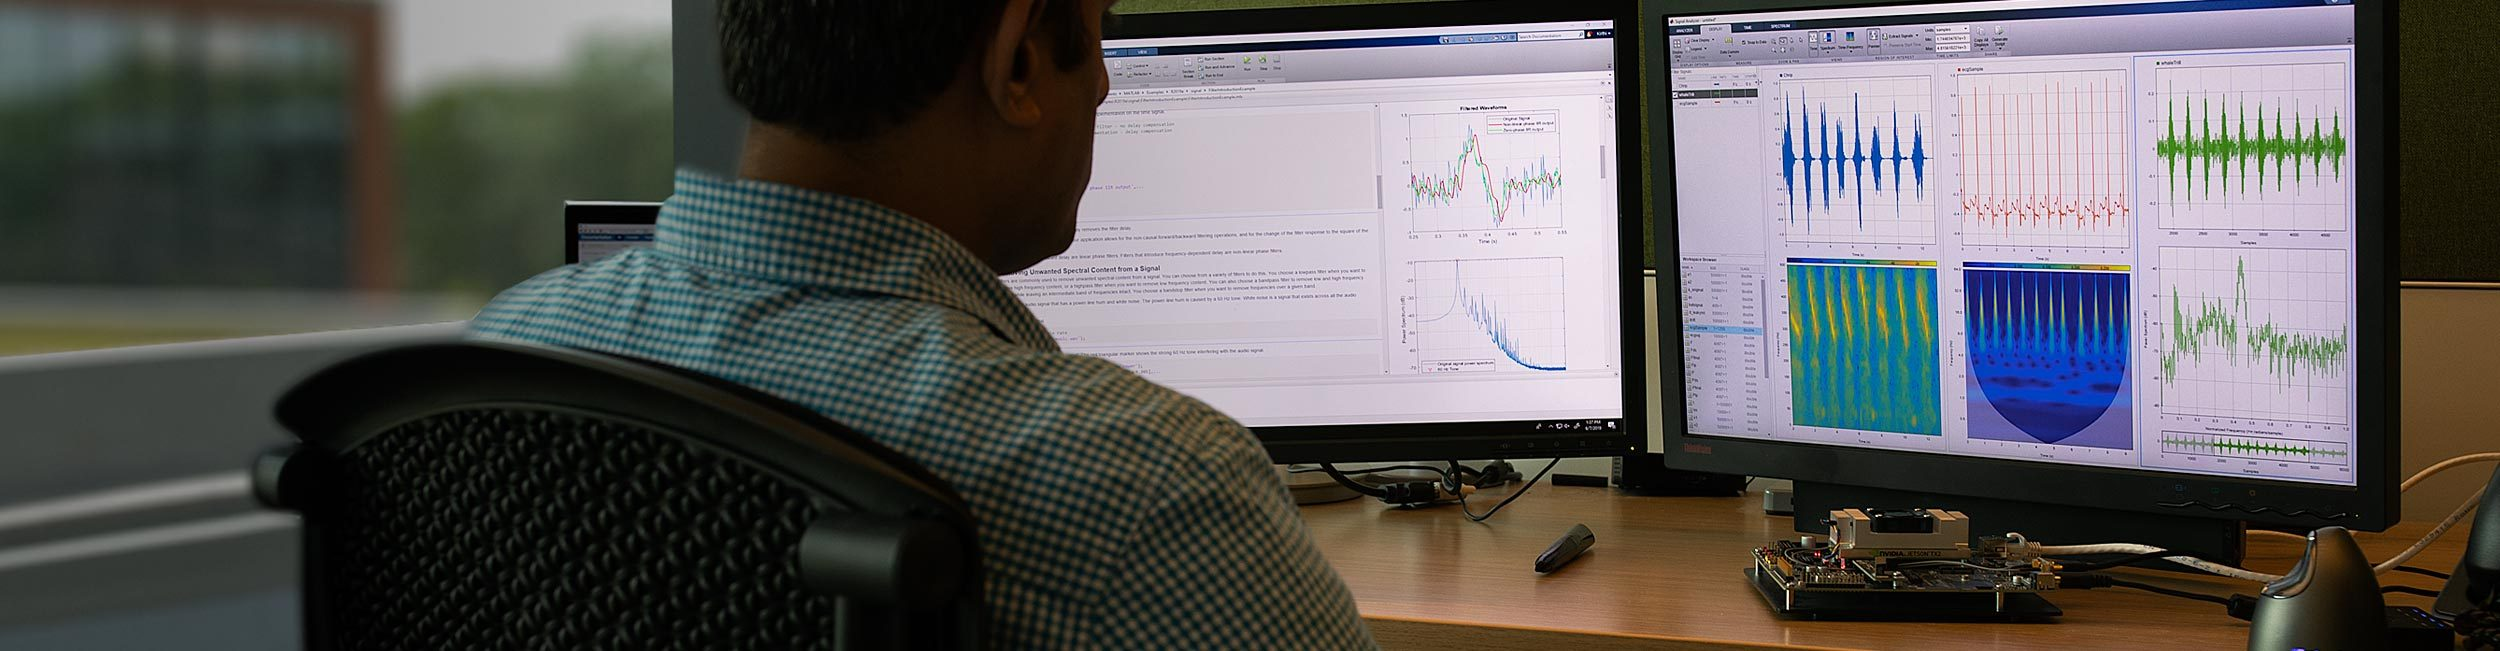
\includegraphics[scale=0.18]{Chapter3/aPersonUsingMATLAB}
\caption{Signal processing engineer using MATLAB and Simulink}
\label{aPersonUsingMATLAB}
\end{center}
\end{figure}
